% Options for packages loaded elsewhere
\PassOptionsToPackage{unicode}{hyperref}
\PassOptionsToPackage{hyphens}{url}
%
\documentclass[
]{article}
\usepackage{amsmath,amssymb}
\usepackage{iftex}
\ifPDFTeX
  \usepackage[T1]{fontenc}
  \usepackage[utf8]{inputenc}
  \usepackage{textcomp} % provide euro and other symbols
\else % if luatex or xetex
  \usepackage{unicode-math} % this also loads fontspec
  \defaultfontfeatures{Scale=MatchLowercase}
  \defaultfontfeatures[\rmfamily]{Ligatures=TeX,Scale=1}
\fi
\usepackage{lmodern}
\ifPDFTeX\else
  % xetex/luatex font selection
\fi
% Use upquote if available, for straight quotes in verbatim environments
\IfFileExists{upquote.sty}{\usepackage{upquote}}{}
\IfFileExists{microtype.sty}{% use microtype if available
  \usepackage[]{microtype}
  \UseMicrotypeSet[protrusion]{basicmath} % disable protrusion for tt fonts
}{}
\makeatletter
\@ifundefined{KOMAClassName}{% if non-KOMA class
  \IfFileExists{parskip.sty}{%
    \usepackage{parskip}
  }{% else
    \setlength{\parindent}{0pt}
    \setlength{\parskip}{6pt plus 2pt minus 1pt}}
}{% if KOMA class
  \KOMAoptions{parskip=half}}
\makeatother
\usepackage{xcolor}
\usepackage[margin=1in]{geometry}
\usepackage{graphicx}
\makeatletter
\def\maxwidth{\ifdim\Gin@nat@width>\linewidth\linewidth\else\Gin@nat@width\fi}
\def\maxheight{\ifdim\Gin@nat@height>\textheight\textheight\else\Gin@nat@height\fi}
\makeatother
% Scale images if necessary, so that they will not overflow the page
% margins by default, and it is still possible to overwrite the defaults
% using explicit options in \includegraphics[width, height, ...]{}
\setkeys{Gin}{width=\maxwidth,height=\maxheight,keepaspectratio}
% Set default figure placement to htbp
\makeatletter
\def\fps@figure{htbp}
\makeatother
\setlength{\emergencystretch}{3em} % prevent overfull lines
\providecommand{\tightlist}{%
  \setlength{\itemsep}{0pt}\setlength{\parskip}{0pt}}
\setcounter{secnumdepth}{5}
\usepackage{booktabs}
\usepackage{longtable}
\usepackage{array}
\usepackage{multirow}
\usepackage{wrapfig}
\usepackage{float}
\usepackage{colortbl}
\usepackage{pdflscape}
\usepackage{tabu}
\usepackage{threeparttable}
\usepackage{threeparttablex}
\usepackage[normalem]{ulem}
\usepackage{makecell}
\usepackage{xcolor}
\ifLuaTeX
  \usepackage{selnolig}  % disable illegal ligatures
\fi
\usepackage[]{natbib}
\bibliographystyle{plainnat}
\IfFileExists{bookmark.sty}{\usepackage{bookmark}}{\usepackage{hyperref}}
\IfFileExists{xurl.sty}{\usepackage{xurl}}{} % add URL line breaks if available
\urlstyle{same}
\hypersetup{
  pdftitle={Hebbian learning can explain rhythmic neural entrainment to statistical regularities},
  pdfauthor={Ansgar D. Endress, City, University of London},
  pdfkeywords={Keywords},
  hidelinks,
  pdfcreator={LaTeX via pandoc}}

\title{Hebbian learning can explain rhythmic neural entrainment to
statistical regularities}
\author{Ansgar D. Endress, City, University of London}
\date{}

\begin{document}
\maketitle
\begin{abstract}
In many domains, continuous sequences are composed of discrete recurring
units. Learners need to extract these recurring units. A prime example
is word learning. Fluent speech in unknown language is perceived as a
continuous signal. Learners need to extract (and then memorize) its
underlying words. One prominent candidate mechanism involves tracking
how predictive syllables (or other items) are of one another, a strategy
formalized as Transitional Probabilities (TPs). Syllables within the
same word are more predictive of one another than syllables straddling
word boundaries. Behaviorally, it is controversial whether such
statistical learning abilities allow learners to extract and store the
underlying units in memory, or whether they just track pairwise
associations among syllables. The strongest evidence for the former view
comes from electrophysiological results, showing evoked responses
time-locked to word boundaries (e.g., N400's) as well as rhythmic
activity with a periodicity of the unit duration. Here, I show that a
simple Hebbian network can explain such results. When exposed to
statistically structured syllable sequences, the network activation is
rhythmic with a periodicity of the word duration and an activation
maximum on word-final syllables. This is because word-final syllables
receive more excitatory input from earlier syllables with which they are
associated than syllables that occur earlier in words (and are less
predictable). Hebbian learning can thus account for rhythmic neural
activity in statistical learning task in the absence of memory
representations for words, and previous reports of N400s time-locked to
word boundaries might index the reduced predictability of word-initial
syllables rather than word-onsets. I also suggest that learners might
need to rely on other cues to extract and learn the words of their
native language.
\end{abstract}

\hypertarget{introduction}{%
\section{Introduction}\label{introduction}}

During language acquisition, word learning is challenging even when the
phonological form of words is known \citep{Gillette1999, Medina2011}.
However, speech in unknown languages often appears as a continuous
signal with few cues to word onsets and offsets (but see
\citep{Brentari2011, Christophe2001, Endress-cross-seg, Johnson2001a, Johnson2009, Pilon1981, Shukla2007, Shukla2011}).
As a result, learners first need to discover where words start and where
they end before than can commit any phonological word form to memory
\citep{Aslin1998, Saffran-Science, Saffran1996b} (and hopefully link it
to some meaning). This challenge is called the segmentation problem.

Learners might solve the segmentation problem using co-occurrence
statistics tracking the predictability of syllables. For example, a
syllable following ``the'' is much harder to predict than a syllable
following ``whis''. After all, ``the'' can precede any noun, but there
are very few words starting with ``whis'' (e.g., whiskey, whisker,
\ldots).

The most prominent version of such co-occurrence statistics involves
Transitional Probabilities (TPs), i.e., the conditional probability of a
syllable \(\sigma_2\) following another syllable \(\sigma_1\)
\(P(\sigma_2|\sigma_1)\). Infants, newborns and non-human animals are
all sensitive to TPs in a variety of modalities
\citep{Aslin1998, Chen2015, Creel2004, Endress-tone-tps, Endress-Action-Axc, Fiser2002a, Fiser2005, Flo2022, Glicksohn2011, Hauser2001, Kirkham2002, Saffran1996b, Saffran-Science, Saffran1999, Saffran2001, Sohail2016, Toro2005-backward, Turk-Browne2005, Turk-Browne-reversal}.

Following \citep{Aslin1998, Saffran-Science, Saffran1996b}, participants
in a typical behavioral statistical learning experiment in the auditory
modality are first familiarized with a statistically structured speech
stream (or a sequence in another modality such as auditory tones or
visual symbols). The speech stream is a random concatenation of triplets
of non-sense syllables (hereafter ``words''). Syllables within words are
thus more predictive of one another than syllable across
word-boundaries. For example, if \emph{ABC}, \emph{DEF}, \emph{GHJ} and
\emph{KLM} are ``words'' (where each letter represents a syllable), the
\emph{C} at the end of \emph{ABC} can be followed by the word-initial
syllables of any of the other words, while syllables within words
predict each other with certainty.

A sensitivity to TPs is then tested by measuring a preference between
high-TP items (i.e., words) and low-TP items created by taking either
the final syllable of one word and the first two syllables from another
word (e.g., \emph{CDE}) or by taking the last two syllables of one word
and the first syllable of the next word (e.g., \emph{BCD}); the low-TP
items are called part-words. Participants (adults, infants or other
animals) usually discriminate between words and part-words, suggesting
that they are sensitive to TPs. In humans, such a sensitivity to TPs
might be the first step towards word learning.

\hypertarget{does-statistical-learning-help-learners-memorizing-words}{%
\subsection{Does statistical learning help learners memorizing
words?}\label{does-statistical-learning-help-learners-memorizing-words}}

While many authors propose that tracking TPs leads to the addition of
words to the mental lexicon (and thus to storage of word candidates in
declarative long-term memory, LTM)
\citep{Erickson2014, Estes2007, Hay2011a, Isbilen2020, Karaman2018, Perruchet2019, Shoaib2018},
the extent to which a sensitivity to TPs really supports word learning
is debated, and the results supporting this view often have alternative
explanations that do not involve declarative LTM (see
\citep{Endress2020, Endress-stat-recall} for critical reviews). For
example, while high-TP items are sometimes easier to memorize than
low-TP items \citep{Estes2007, Hay2011a, Isbilen2020, Karaman2018}, it
is unclear if any LTM representation have been formed during statistical
learning, or whether statistical associations simply facilitate
subsequent associations. Likewise, while incomplete high-TP items are
sometimes harder to recognize than entire items, such results can be
explained by memory-less Hebbian learning mechanisms, and other
attentional accounts \citep{Endress-stat-recall}.

Critically, to the extent that a sensitivity to TPs relies on implicit
learning mechanisms \citep{Christiansen2018, Perruchet2006}, statistical
learning might be dissociable from explicit, declarative memory
(\citep{Cohen1980, Finn2016, Graf1984, Knowlton1996a, Poldrack2001, Sherman2020, Squire1992};
though different memory mechanisms can certainly interact during
consolidation \citep{Robertson2022}). In fact, there is evidence that a
sensitivity to TPs is \emph{not} diagnostic of the addition of items to
the mental lexicon. For example, observers sometimes prefer high-TP
items to low-TP items when they have never encountered either of them
(when the items are played backwards compared to the familiarization
stream; \citep{Endress-Action-Axc, Turk-Browne-reversal, Jones2007}),
and sometimes prefer high-TP items they have never encountered over
low-TP items they have heard or seen
\citep{Endress-Phantoms-Vision, Endress-Phantoms}. In such cases, a
preference for high-TP items does not indicate that the high-TP items
are stored in the mental lexicon, simply because learners have never
encountered these items. Further, when learners have to repeat back the
items they have encountered during a familiarization stream with as few
as four items, they are unable to do so \citep{Endress-stat-recall}.

On the other hand, there is a straightforward explanation of such
results that does not involve declarative LTM: a sensitivity to TPs
might reflect Hebbian learning
\citep{Endress-tone-tps, Endress-TP-Model}. After all, the
representations of syllables (or other elements in a stream) presumably
does not cease to be active as soon as the syllable ends. As a result,
multiple syllables can be active together and can can thus form Hebbian
associations. \citep{Endress-TP-Model} showed that such a network can
account for a number of statistical learning results (see below).

However, there is another class of studies that seems to provide strong
evidence for the possibility that statistical learning leads to the
extraction of coherent units, and that seems to be inconsistent with a
mere Hebbian interpretation of statistical learning results:
electrophysiological responses to statistically structured sequences. I
will now turn to this literature.

\hypertarget{electrophysiological-correlates-of-statistical-learning}{%
\subsection{Electrophysiological correlates of statistical
learning}\label{electrophysiological-correlates-of-statistical-learning}}

In one of the earliest electrophysiological studies of statistical
learning, \citep{Sanders2002} first presented participants with a speech
stream composed of non-sense words. Following this, they presented these
words in isolation, and finally another speech stream with the same
words. When they compared electrical brain responses to the second
presentation of the stream and its first presentation, they observed
increased N100 and N400 responses. That is, they showed increased
negativities around 100 ms and 400 ms after word onsets (see also
\citep{Abla2008} for similar study with tones rather than syllables as
stimuli). \citep{Cunillera2006} showed that N400 effects can also be
obtained without explicitly training participants on the words, and
similar results obtain even in newborns \citep{Kudo2011, Teinonen2009}.

Following \citep{Buiatti2009}, electrophysiological investigations of
statistical learning focused on rhythmic entrainment to the speech
streams rather than event-related responses such as the N400.
Specifically, if listeners learn the statistical structure of the speech
stream, they should perceive the speech stream as a sequence of
trisyllabic units (given that most statistical learning experiments tend
to use tri-syllabic units or their equivalents in other domains, but see
\citep{Johnson2010}), and thus perceive a rhythm with a periodicity of
three syllable durations. If so, they should also show a \emph{neural}
rhythm with the same periodicity. While \citep{Buiatti2009} detected
such a rhythm only when words were separated by brief silences, later
investigations found such rhythms in continuous sequences in adults
\citep{Batterink2017} (see also \citep{Moser2021} for an
magneto-encephalography study), children \citep{Moreau2022}, infants
\citep{Kabdebon2015} and even newborns \citep{Flo2022}.

Such results seem to strongly suggest that statistical learning creates
integrated units that can (presumably) be stored in memory, and
different authors have reached this conclusion
\citep{Batterink2017, Flo2022, Sanders2002, Teinonen2009}. However, the
original interpretation of the N400 component suggests a different
interpretation. In fact, the electrical N400 component is thought to
reflect (semantically) surprising and thus unpredictable stimuli
\citep{Kutas2000}. However, in speech streams such as those used in
statistical learning tasks, word onsets are always unpredictable, given
that words are randomly concatenated, and word onsets remain
unpredictable even when participants learn the statistical structure of
the speech stream. As a result, it is unclear why N400-like responses
should be time-locked to word \emph{onsets.} In contrast, the last
syllable of each word is predictable based on the statistical structure
of the streams, but only after learning. As a result,
electrophysiological responses might not so much index word onsets as
reflect the increased predictability of word-final syllables (or the
decreased relative predictability of word-initial syllables) as learning
progresses.

A similar conclusion follows from simple associative considerations. For
example, after a word \emph{ABC} is learned (where each letter stands
for a syllable), each syllable predicts subsequent syllables. As a
result, the \emph{C} syllable does not only receive (external) bottom-up
excitation when it is encountered, but receives additional associative
excitation from the preceding \emph{A} and \emph{B} syllables (that
predict the \emph{C} syllable). As a result, one would expect a neural
rhythm with a period of three syllable durations, and a maximum
following the onset of the \emph{word-final} syllable even if no word
has been stored in memory.

\hypertarget{the-current-study}{%
\section{The current study}\label{the-current-study}}

Here, I provide computational evidence for this idea, and show that such
electrophysiological results can be explained in a simple, memory-less
Hebbian network that has been used to account for a variety of
statistical learning results \citep{Endress-TP-Model}. The network is a
fairly generic saliency map
\citep{Bays2010, Endress-Catastrophic-Interference, Gottlieb2007, Roggeman2010, Sengupta2014}
augmented by a Hebbian learning component. The network comprises units
representing populations of neurons encoding syllables (or other items).
All units are fully connected with both excitatory and inhibitory
connections. Excitatory connections change according to a Hebbian
learning rule, while inhibitory connections do not undergo learning.
Additionally, activation decays exponentially in all units. Further
details of the model can be found in Supplementary Information XXX.

\begin{figure}
\centering
\includegraphics{figures/network_schema.pdf}
\caption{Illustration of the network architecture with only three units
\emph{A}, \emph{B} and \emph{C}. Here, these units encode syllable. All
units mutually exite and inhibit one another. Excitatory connections
undergo Hebbian learning. For example, unit \emph{A} excites unit
\emph{B} with a tunable weight of \(w_{BA}\) as well as unit \emph{C}
with a weight of \(w_{CA}\). In contrast, the inhibitory weight does not
undergo learning. In addition to excitation and inhibition, all units
undergo forgetting.}
\end{figure}

Such an architecture can explain statistical learning results in a
relatively intuitive way. For example, if each syllable is represented
by some population of neurons, and learners listen to some sequence
\emph{ABCD}\ldots, associations should form between adjacent and
non-adjacent syllables depending on the decay rate. If activation decay
is slower than a syllable duration, the representations of two adjacent
syllables will be active at the same time, and thus form an association.
For example, if a neuron representing \emph{A} is still active while
\emph{B} is presented, these neurons can form an association. Similarly,
if a neuron representing \emph{A} is still active when \emph{C} is
presented, an association between these neurons will ensue although the
corresponding syllables are not adjacent.

Further, this learning rule is non-directional. As a result, the network
should be sensitive to associations irrespective of whether items are
played in their original order (e.g., \emph{ABC}) or in reverse order
(e.g., \emph{BCA}). \citep{Endress-TP-Model} showed that such a model
can account for a number of statistical learning results (as long as the
decay rate was set to a reasonable level) - in the absence of a
dedicated memory store. Hence, statistical learning results can be
explained even when participants do not create lexical entries for
high-TP items.

However, the neural entrainment results above seem to suggest that
learners do more than merely computing associations among syllables, and
extract statistically coherent units
\citep{Batterink2017, Flo2022, Sanders2002, Teinonen2009}. Here, I argue
that this simple Hebbian network can also account for the periodic
activity found in electrophysiological recordings. Intuitively, if a
high-TP item such as \emph{ABC} is presented, \emph{A} mostly receives
external stimulation, but \emph{B} receives external stimulation -- as
well as excitatory input from \emph{A}, while \emph{C} receives external
stimulation as well as excitatory input from both \emph{A} and \emph{B}.
As a result, the network activation should increase towards the end of a
word, with a maximum on the third syllable, leading to periodic activity
with a period of a word duration (though the presence of inhibitory
connections might make the exact results more complex). If so, and as
mentioned above, previous reports of N400 near a word boundary would not
so much indicate the onset of a ``word'', but rather the onset of a
``surprising'' syllable.

I tested this idea in \citep{Endress-TP-Model} model. I exposed the
network to a continuous sequence inspired by \citep{Saffran-Science}
Experiment 2. The sequence consisted of 4 distinct words of 3 syllables
each. The familiarization sequence was a random concatenations of these
words, with each word occurring 100 times. During the test phase, I
recorded the total network activation as each of the test-items (see
below) is presented, and assume that this activation reflects the
network's familiarity with the words.\footnote{\citep{Endress-TP-Model}
  also reported simulations where they recorded the activation in the
  items comprising the current test-item rather than the global network
  activation. While the results were very similar to those using the
  total network activation, measuring activation in test items would not
  be meaningful in the current simulations as I seek to uncover periodic
  activity during familiarization.} I simulated 100 participants by
repeating the familiarization and test cycle 100 times.

The test items follow by \citep{Saffran-Science} and
\citep{Saffran1996b}, among many others. After exposure to the
familiarization sequence, activation is recorded in response to words
such as \emph{ABC} and ``part-words.'' As mentioned above, part-words
comprise either the last two syllables from one word and the first
syllable from the next word (e.g., \emph{BC:D}, where the colon
indicates the former word boundary that is not present in the stimuli)
or the last syllable from one word and the first two syllables from the
next word (e.g., \emph{C:DE}). Part-words are thus attested in the
familiarization sequence, but straddle a word boundary. As a result,
they have weaker TPs than words. Accordingly, the network should be more
familiar with words than with part-words. To assess whether the network
can also account for results presented by \citep{Flo2022} (see below), I
also record activation after presenting the first two syllables of a
word (e.g., \emph{AB}) or the last two syllables (e.g., \emph{BC}).

During the simulations, the network parameters for self-excitation and
mutual inhibition are kept constant (\(\alpha\) and \(\beta\) in
Supplementary Material XXX). However, in line with
\citep{Endress-TP-Model}, I used different forgetting rates
(\(\lambda_{act}\) in Supplementary Material XXX) between 0.1, 0.2, 0.3,
0.4, 0.5, 0.6, 0.7, 0.8, 0.9. With exponential forgetting, a forgetting
rate of 1 means that the activation completely disappears on the next
time step (in the absence of excitatory input), a forgetting rate of
zero means no forgetting at all, while a forgetting rate of .5 implies
the activation is halved on the next time step (again, in the absence of
excitatory input).\footnote{While I use the label ``decay'', I do not
  claim that ``decay'' reflects a psychological processes. The current
  implementation uses decay as a mechanism to limit activations in time,
  but the same effect could likely be obtained through inhibitory
  interactions or other mechanisms.}

\clearpage

\hypertarget{results}{%
\section{Results}\label{results}}

\hypertarget{preference-for-words-over-part-words}{%
\subsection{Preference for words over
part-words}\label{preference-for-words-over-part-words}}

To establish the forgetting rates at which discrimination between words
and part-words (and thus learning) can be observed, I first repeat some
of \citep{Endress-TP-Model} results. I calculated normalized difference
scores of activations for words and part-words,
\(d = \frac{\text{Word} - \text{Part-Word}}{\text{Word} + \text{Part-Word}}\),
and evaluated these difference scores in two ways. First, I comparde
them to the chance level of zero using Wilcoxon tests. Second, I counted
the number of simulations (representing different participants)
preferring words, and evaluated this count using a binomial test. With
100 simulations per parameter set, performance is significantly
different from the chance level of 50\% if at least 61 \% of the
simulations show a preference for the target items.

\begin{figure}
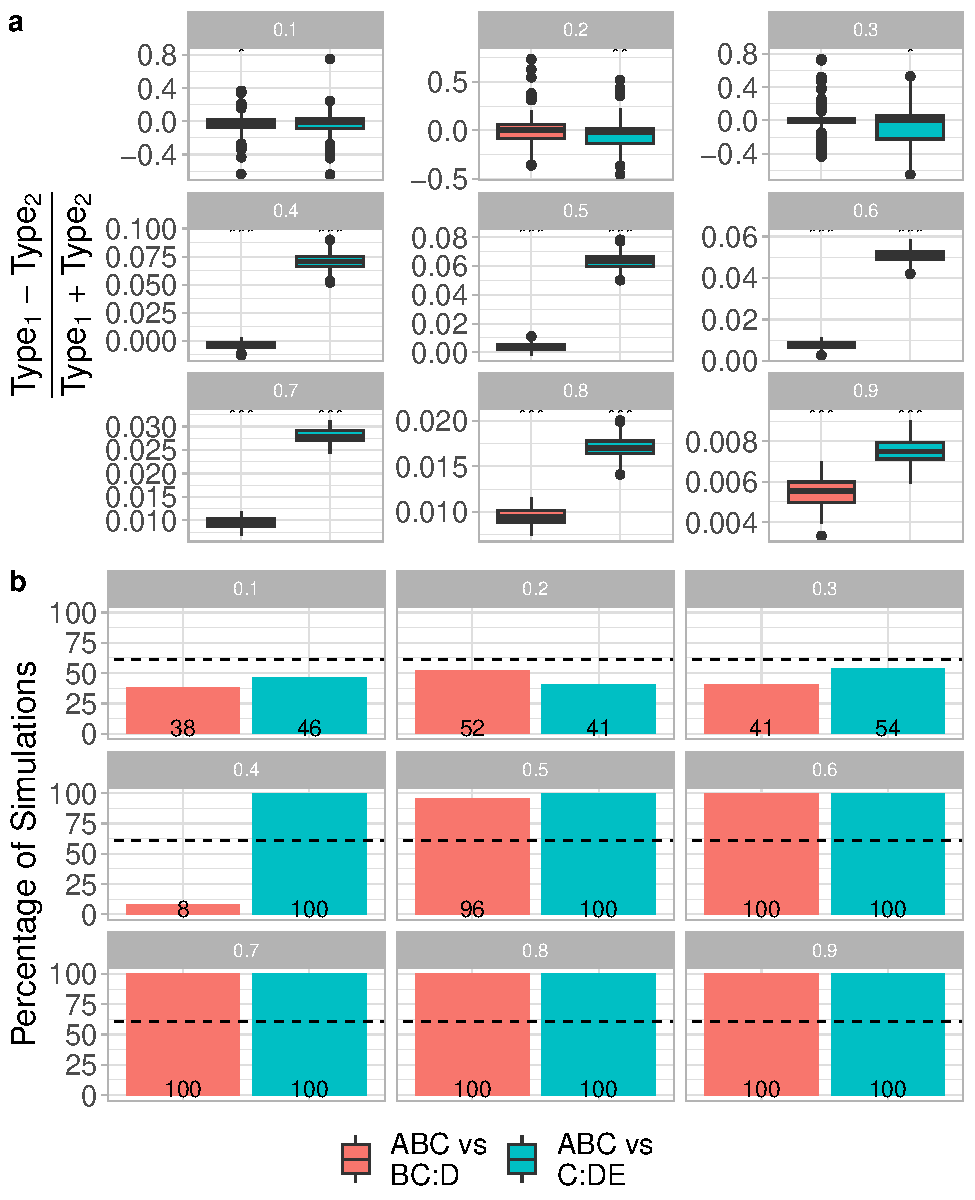
\includegraphics[width=1\linewidth]{tp_model_entrainment_files/figure-latex/basic-experiment-global-create-plot-combined-fw-plot-1} \caption{Results based on the global activation as a measure of the network's familiarity with the items for forgetting rates (between 0.1 and 0.9). (a) Difference scores between words and part-words. Significance is assessed based on Wilcoxon tests against the chance level of zero. (b) Percentage of simulations with a preference for words over part-words. The dashed line shows the minimum percentage of simulations that is significant based on a binomial test.}\label{fig:basic-experiment-global-create-plot-combined-fw-plot}
\end{figure}

The results are shown in Figure
\ref{fig:basic-experiment-global-create-plot-combined-fw-plot} and Table
\ref{tab:basic-experiment-global-evaluate-diff-print2}. Except for low
forgetting rates of up to .4, the network prefers words over part-words,
with somewhat better performance for words against \emph{C:DE}
part-words, as has been observed in human participants by
\citep{Fiser2002}. In the following, I will thus use forgetting rates
between 0.4 and 0.9 to model the electrophysiological results.

\clearpage

\hypertarget{electrophysiological-results}{%
\subsection{Electrophysiological
results}\label{electrophysiological-results}}

\hypertarget{activation-differences-within-words}{%
\subsubsection{Activation differences within
words}\label{activation-differences-within-words}}

I next asked whether a basic Hebbian learning model can explain periodic
activity found in electrophysiological recordings
\citep{Buiatti2009, Batterink2017, Flo2022, Kabdebon2015, Moreau2022, Moser2021},
focusing on the forgetting rates for which the network preferred words
to part-words. In a first analysis, I simply recorded the total network
activation after each syllable in a word had been presented. These
activations were averaged for each syllable position (word-initial,
word-medial and word-final) and for each participant after removing the
first 200 words from the familiarization stream (during which the
network was meant to learn).

As shown in Figure
\ref{fig:basic-experiment-global-print-act-in-words-plot} and Table
\ref{tab:basic-experiment-global-print-act-in-words-table2}, activation
was highest after word-final syllables (though not for very low
forgetting rates for which I did not observe learning in the first
place). As a result, a simple Hebbian learning model can account for
rhythmic activity in electrophysiological recordings with a period
equivalent to the word duration. Critically, and as mentioned above,
while previous electrophysiological responses to statistical structured
streams were interpreted in terms of a response to word onsets
\citep{Abla2008, Cunillera2006, Kudo2011, Sanders2002, Teinonen2009},
the current results suggest an alternative interpretation of such
effects. Rather than signalling the beginnings and ends of words, an
activation maximum after the third syllable of each word might reflect
the predictability of the third syllable, while a sudden drop in
activation after the first syllable might indicate the lack of
predictability. Importantly, such activation maxima can arise even if no
word is stored in memory.

The reason for which lower forgetting rates do not necessarily lead to
rhythmic activity is the interplay between decay and inhibition. To
assess this possibility, I recorded the number of active neurons after a
burn-in phase of 600 items. As shown in Table
\ref{tab:inspect-number-of-active-neurons-print2} and Figure
\ref{fig:inspect-number-of-active-neurons-plot2}, more neurons remain
active at any point in time when the decay rate is lower, and might thus
inhibit other neurons. When decay limits the effect of residual
inhibitory input from other neurons, the pattern of connections between
neurons then enables the network to exhibit periodic activity.

\begin{figure}
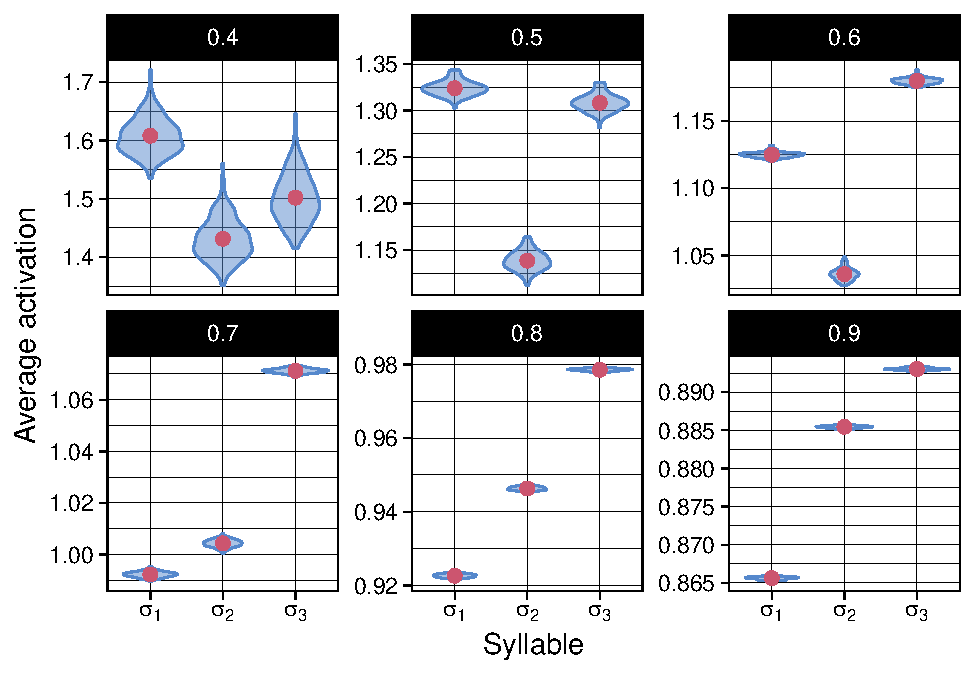
\includegraphics[width=1\linewidth]{tp_model_entrainment_files/figure-latex/basic-experiment-global-print-act-in-words-plot-1} \caption{Average total network activation for different syllable positions during the familiarization with a stream following cite{Saffran-Science}. The facets show different forgetting rates. The results reflect the network behavior after the first 50 presentations of each word.}\label{fig:basic-experiment-global-print-act-in-words-plot}
\end{figure}

\hypertarget{spectral-density}{%
\subsubsection{Spectral density}\label{spectral-density}}

I next analyzed the frequency response of the network to the speech
streams. Specifically, I estimated the spectral density of the time
series corresponding to the total network activation after each time
step (again after a burnin of 200 words), separately for each decay rate
and simulation. I then extracted the frequency with the maximal density.
As shown in Figure
\ref{fig:basic-experiment-global-print-freq-phase-plot}(a), the modal
frequency for decay rates of least .4 was 1/3, corresponding to a period
of three syllables. These results thus suggest again that a simple
Hebbian learning mechanism can entrain to statistical rhythms in the
absence of memory for words.

\hypertarget{phase-analysis}{%
\subsubsection{Phase analysis}\label{phase-analysis}}

The analyses of the network activations suggest that activations are
strongest for word-final syllables, and that the network entrains to a
periodicity of three syllables. However, the traditional interpretation
of electrophysiological responses to statistical learning is that neural
responses index word-initial syllables. To address this issue more
directly, I calculated the phase of the network activation relative to
wave forms with maxima on word-initial, word-medial and word-final
syllables, respectively. Specifically, I calculated the cross-spectrum
phase at the winning frequency between the total network activation and
(1) three cosine reference waves with their maxima on the first, second
or third syllable of a word as well as (2) a saw-tooth function with its
maximum on the third syllable. As shown in Figure
\ref{fig:basic-experiment-global-print-freq-phase-plot}(b) and Table
\ref{tab:basic-experiment-global-phase-table2}, the activation had a
small relative phase relative to the cosine with the maximum on the
third syllable or the saw tooth function. In contrast the phase relative
to the cosine with the word-initial maximum was around 120 degrees,
while that relative to the cosine with the maximum on the second
syllable was around -120 degrees. These spectral analyses thus confirm
that, at least for larger decay rates, the activation increases towards
the end of a word, and that the network activation is roughly in phase
with a function with a maximum on the third syllable.

\begin{figure}
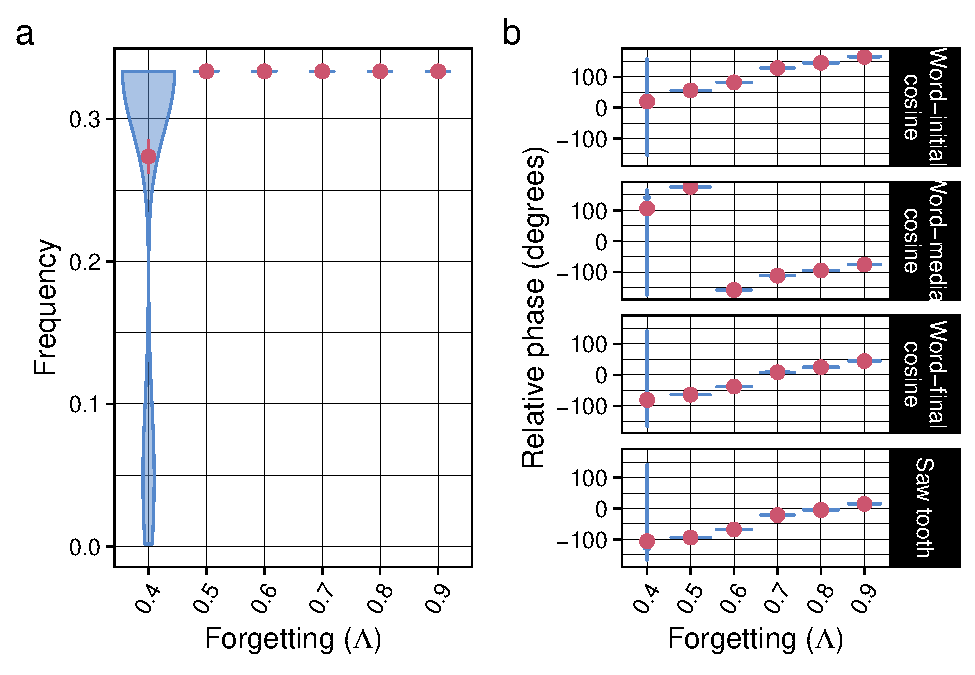
\includegraphics[width=1\linewidth]{tp_model_entrainment_files/figure-latex/basic-experiment-global-print-freq-phase-plot-1} \caption{Spectral analysis of the total network activation during the familiarization with a stream following cite{Saffran-Science}. The results reflect the network behavior after the first 50 presentations of each word. (a) Maximal frequency as a function of the forgeting rates. For forgetting rates where learning takes place, the dominant frequency is 1/3, and thus corresponds to the word length. (b) Relative phase (in degrees) at the maximal frequency of the total network activation relative to (from top to bottom) a cosine function with its maximum at word-intial syllables, word-medial syllables and word-final syllables as well as a saw tooth function with the maximum on the third syllable. For forgetting rates where learning takes place, the total activation is in phase with a cosine with its maximum on the word-final syllable as well as with the corresponding saw tooth function.}\label{fig:basic-experiment-global-print-freq-phase-plot}
\end{figure}

\hypertarget{memory-for-word-onsets-vs.-offsets-flo2022}{%
\subsubsection{\texorpdfstring{Memory for word onsets vs.~offsets
\citep{Flo2022}}{Memory for word onsets vs.~offsets {[}@Flo2022{]}}}\label{memory-for-word-onsets-vs.-offsets-flo2022}}

The results so far suggest that a simple Hebbian network can reproduce
rhythmic activity in the absence of memory for words. However,
\citep{Flo2022} suggested that neonates retain at least the first
syllable of statistical defined words, if not the entire words.
Specifically, they presented newborns with items starting with two
syllables that occurred word-initially (\emph{AB}\ldots), and with items
starting with a word-medial syllable (\emph{BC}\ldots) and observed
early ERP differences between these items.

To reproduce these results, I measured the activation of the network in
response to isolated, bisyllabic \emph{AB} and \emph{BC} test items,
respectively. As shown in Figure
\ref{fig:basic-experiment-global-print-act-after-2syll-plot} and Table
\ref{tab:basic-experiment-global-print-difference-between-parts-of-word2},
the network activation was always greater in response to \emph{BC} items
than to \emph{AB} items except for the largest decay rates. The reasons
is presumably that \emph{BC} associations are somewhat stronger than
\emph{AB} associations, thus leading to more spreading activation. Be
that as it might, these analyses show that a memory-less system can
reproduce differential responses to \emph{AB} and \emph{BC} items.

\begin{figure}
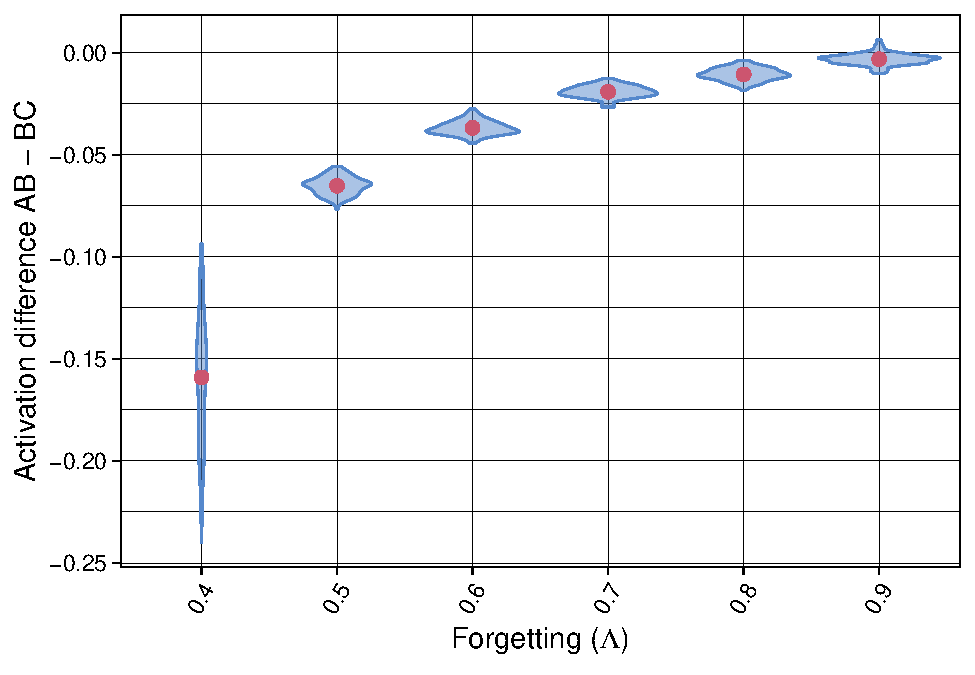
\includegraphics[width=1\linewidth]{tp_model_entrainment_files/figure-latex/basic-experiment-global-print-act-after-2syll-plot-1} \caption{Average difference in the total network activation for the first two syllables of a word (AB) and the first to syllables of a part-word (BC) after familiarization with a stream following cite{Saffran-Science}. The results reflect the network behavior after the first 50 presentations of each word. Positive values indicate greater activation for the AB items than the BC items.}\label{fig:basic-experiment-global-print-act-after-2syll-plot}
\end{figure}

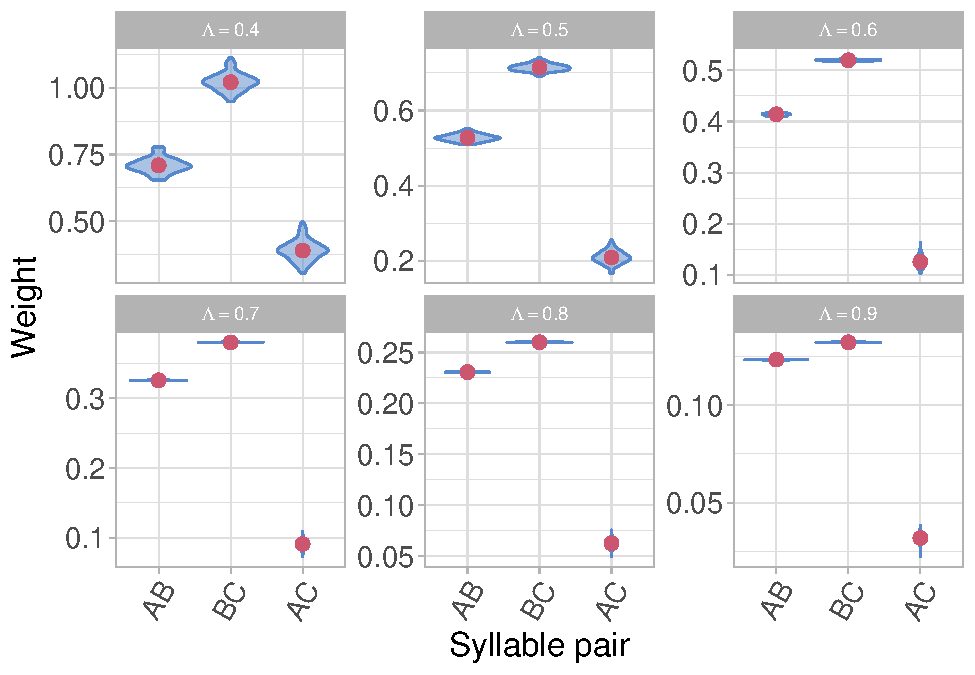
\includegraphics[width=1\linewidth]{tp_model_entrainment_files/figure-latex/basic-experiment-global-print-weights-after-2syll-plot-1}

\begin{figure}
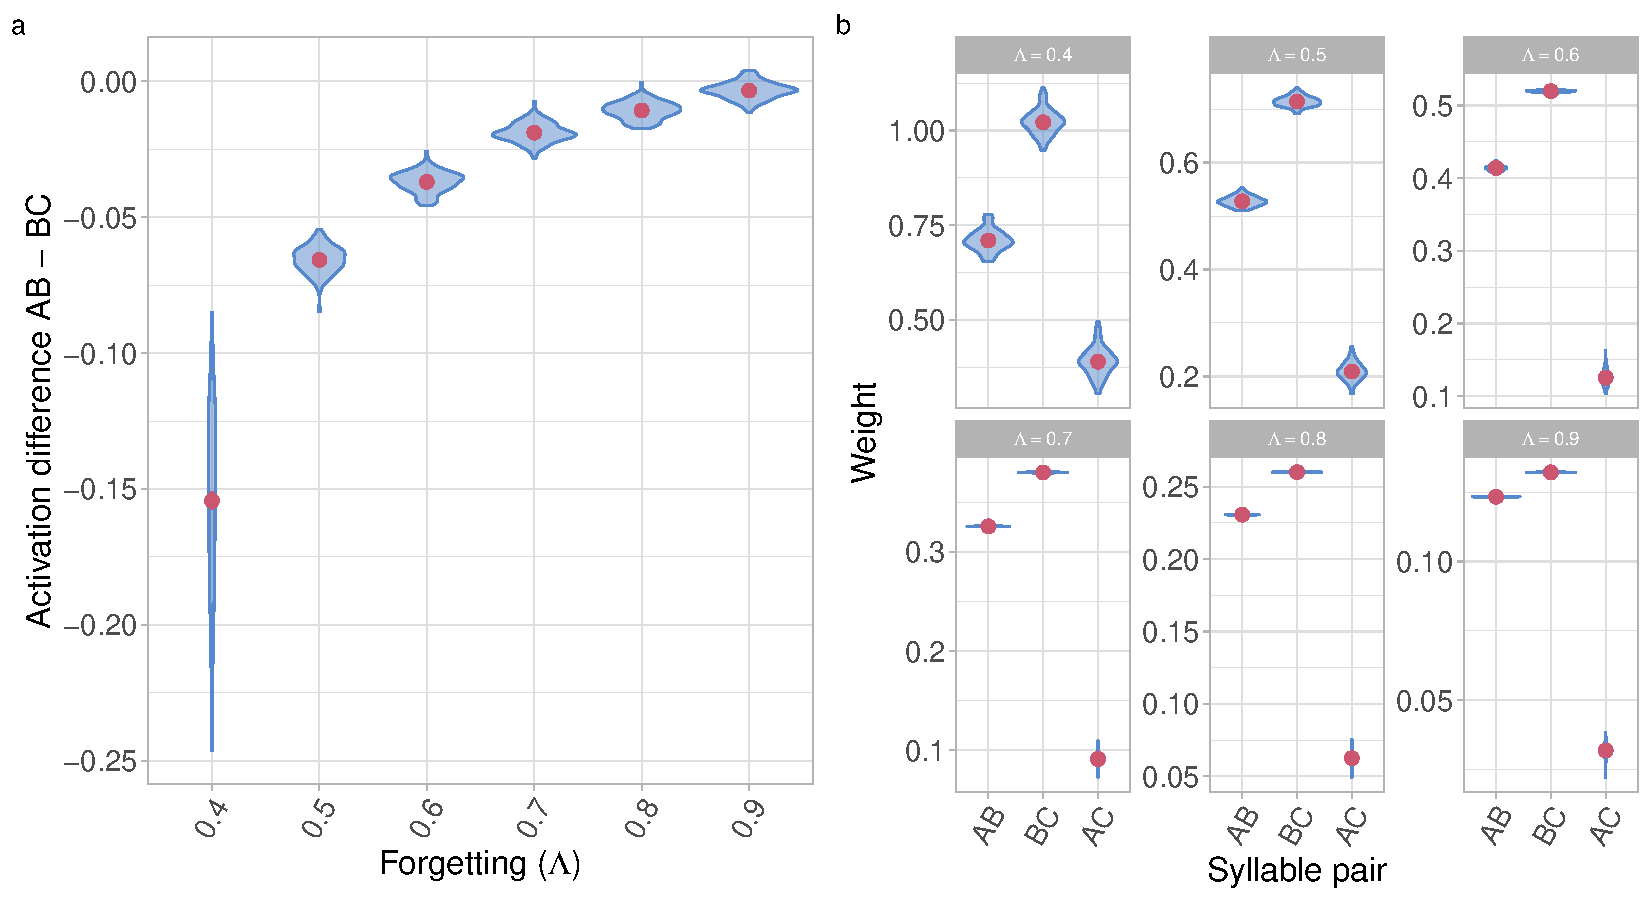
\includegraphics[width=1\linewidth]{tp_model_entrainment_files/figure-latex/basic-experiment-global-print-act-and-weight-after-2syll-plot-1} \caption{(a) Average difference in the total network activation for the first two syllables of a word (AB) and the first to syllables of a part-word (BC) after familiarization with a stream following cite{Saffran-Science}. The results reflect the network behavior after the first 50 presentations of each word. Positive values indicate greater activation for the AB items than the BC items. (b) After familiarization, the connection weight between B and C syllables is somewhat higher than that between A and B items.}\label{fig:basic-experiment-global-print-act-and-weight-after-2syll-plot}
\end{figure}

\clearpage

\hypertarget{positional-coding-new-in-revision}{%
\subsubsection{Positional coding (NEW IN
REVISION)}\label{positional-coding-new-in-revision}}

Other investigators used electrophysiological recordings to reveal more
abstract information extracted from statistically structured sequences.
For example, \citep{Henin2021} found that, in intracranial recordings,
the representations of items sharing a sequential position within words
(i.e., word-initial, word-medial or word-final) were more similar than
the representations of items from different positions, and concluded
that this representational similarity might support positional codes.

However, behavioral evidence suggests that such positional codes are not
available after familiarizations with continuous sequences (e.g.
\citep{Marchetto2013, Endress-AXC, Endress-AXC-Edge, Endress-AXC-Review, Pena2002}),
raising the question of whether this similarity is behaviorally relevant
for learning.

Here, I thus suggest an alternative explanation: The positional
similarity might be a side effect of associative processing.
Specifically, items in the same sequential position share their context.
For example, all word-initial syllables are surrounded by the same set
of word-final syllables and vice-versa. If so, and if the context and
the focal syllables activate each other, one would expect a certain
degree of representational overlap of syllables sharing a sequential
position, without this necessarily having behavioral consequences.

To evaluate this idea, I extracted the activation in all neurons in all
time steps (after burn in). I then calculated, for each forgetting rate,
simulated participant and syllable, the average activation in all
neurons. I then extracted the ``representation'' of all syllables, that
is, the vector of activations observed after a syllable has been
presented. I calculated the cosine similarity across the representations
of all syllable pairs (i.e., the normalized dot product), and calculated
an average similarity for each forgetting rate, simulated participant
and match type (positional match vs.~non-match). Finally, I calculated,
for each forgetting rate and simulated participant, the relative
similarity difference for non-matching vs.~matching pairs,
\(\frac{\text{non-match} - \text{match}}{\text{non-match} + \text{match}}\)
and evaluated these difference scores with a Wilcoxon test against the
chance level of zero.

\begin{figure}
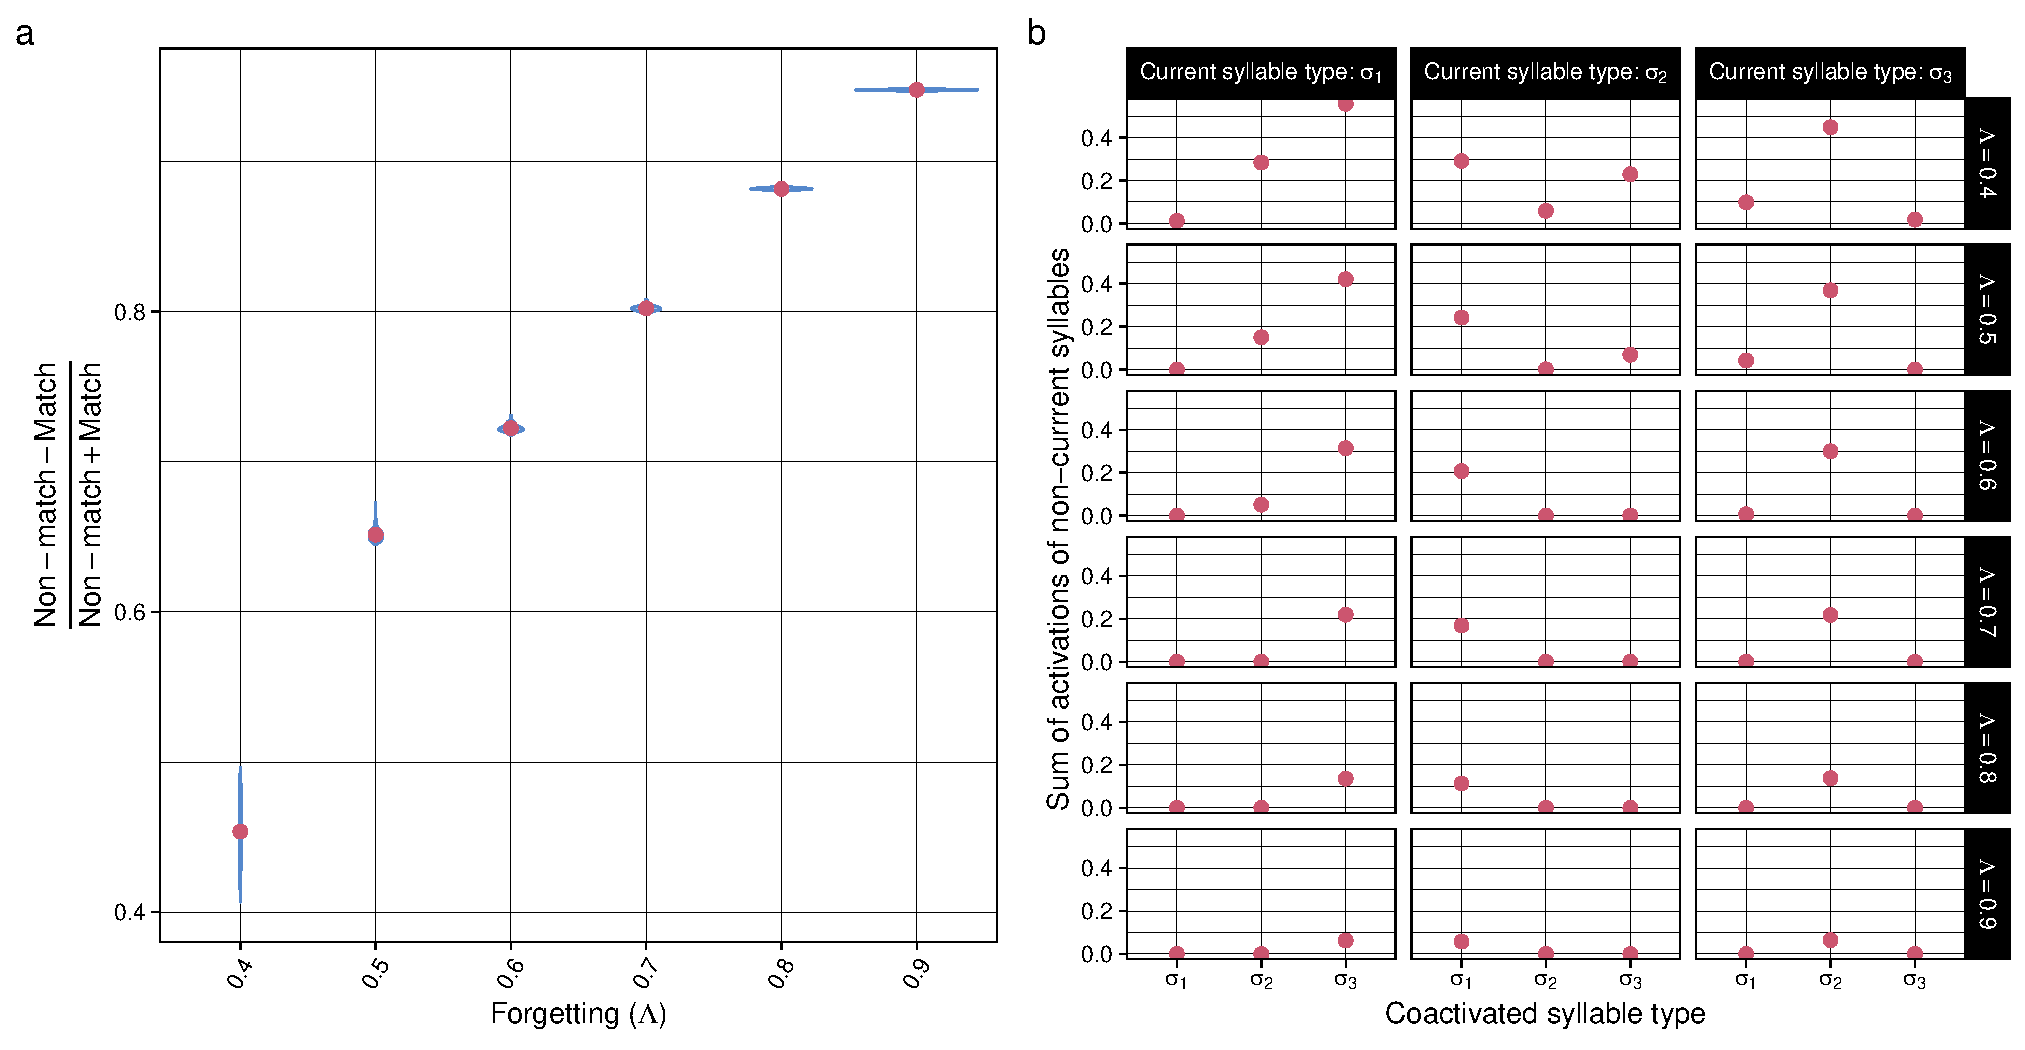
\includegraphics[width=1\linewidth]{tp_model_entrainment_files/figure-latex/basic-similarity-by-position-plot-difference-and-coactivation-1} \caption{(a) Simulations of positional codes cite{Henin2021}. Representations of syllables *not* sharing a sequential position (i.e., word-initial, word-medial, word-final) are more similar to each other than representations of syllables sharing a sequential position. The similarity was evaluated using the cosine similarity across the vectors of activation elicited by the syllables. (b) Sum of co-activations during presentations of word-initial, -medial and -final syllables (columns) of syllables in different sequential positions (x-axis), for different forgetting rates (rows). Most concurrently activated syllables occupy a different sequential position than the currently presented syllable.}\label{fig:basic-similarity-by-position-plot-difference-and-coactivation}
\end{figure}

As shown in Figure
\ref{fig:basic-similarity-by-position-plot-difference-and-coactivation}a
and Table \ref{tab:basic-similarity-by-position-print-difference2}, the
similarity score for non-match pairs was significantly higher than for
match pairs for all forgetting rates. As mentioned above, the reason for
this result is likely the types of syllables that are co-activated.

To illustrate this idea, I summed the activations of all other syllables
while a focal syllable was presented. For example, while the
word-initial syllable \emph{A} was presented, I separately summed the
activations of all other word-initial syllables (excluding \emph{A}
itself), all word-medial syllables, and all word-final syllables, and
averaged these sums for all (word-initial, word-medial or word-final)
syllable types. As shown in Figure
\ref{fig:basic-similarity-by-position-plot-difference-and-coactivation}b,
there was little co-activation between syllables of the same type. In
contrast, during presentation of word-initial syllables, word-final
syllables were fairly active; during presentation of word-medial
syllables, word-initial syllables were relatively active, while
word-final syllables were co-activated with word-medial syllables. In
other words, the positional similarity in syllable representations is
due to the context in which these syllables occur, and not due to
positional codes.

The reason for the inversion of the sign of the difference with respect
to \citep{Henin2021} is presumably the time course in the current model
vs.~in actual biological tissue. In the current simulations, a syllable
duration is a discrete time-step. The activations reported here are thus
snapshots of more continuously evolving activations. As a result, the
representations of, say, word-initial and word-final syllables overlap,
given that these syllables excite each other in the same time step. In
contrast, given the localist coding scheme used here, there is no
overlap in the representations of syllables occupying the same
sequential position.

In contrast, with realistic activation time courses, the time-resolved
similarity measures used by \citep{Henin2021} can capture the actual
time course of the associative activation. For example, upon
presentation of a word-initial syllable, such measures can capture any
lingering activation of the representations of the previous word-final
syllable as well as its reactivation through excitation from the
word-initial syllable. I surmise that these time series make the same
same-position representations more similar. Be that as it might, the
current model can differentiate between different sequential positions.

Given that, behaviorally, the positional codes do not seem to be
available to actual learners, the current results also suggest that
caution is required when interpreting information that can be decoded
from the brain without being behaviorally relevant. To take a
non-psychological example, audio recordings often contain noise from the
electric grid from which spatial and temporal localization information
can be decoded (e.g., for forensic purposes \citep{Grigoras2005}).
However, while this information is clearly present in the recordings, it
is not relevant for the primary means by which audio information is
consumed (i.e., by listening to it). Mutatis mutandis, some information
might be present in neural activity as a side effect of the mechanics of
neural processing, but whether this information is behaviorally relevant
is an independent and empirical question.

\hypertarget{effects-of-word-length-new-in-revision}{%
\subsubsection{Effects of word length (NEW IN
REVISION)}\label{effects-of-word-length-new-in-revision}}

I next asked whether the network can entrain to statistical regularities
when the familiarization streams are composed of words of arbitrary
length. Intuitively, given that the periodicity reported here arises due
to the increasing cumulative excitatory input towards the ends of words,
one would expect the network to be unable to track statistical
periodicity for excessively long words. After all, for sufficiently long
words, the activation from to earlier syllables will have disappeared
once the input reaches the end of a word.

There is some evidence supporting this idea. For example,
\citep{Benjamin2023} did not find neural entrainment to 4-syllable words
in newborns (though a failure to detect entrainment might have other
reasons than the word length.) Computationally, however, it is also
conceivable that networks can deal with longer words, if spreading
activation due to higher order associations are sufficient to increase
the network activation towards the end of a word.

To examine this issue, I repeated the simulations above, but with word
lengths between 3 and 18 syllables, again for the same forgetting rates
as in the simulations above and 100 simulated participants. I estimated
the spectral density of the time series corresponding to the total
network activation after each time step (again after a burnin of 200
words), separately for each decay rate and simulation. I then extracted
the frequency with the maximal density, and averaged these frequencies
across participants.

As shown in Figures
\ref{fig:basic-experiment-global-by-n-syll-create-freq-plot} and
\ref{fig:basic-experiment-global-by-n-syll-modal-freq-plot}, the network
successfully tracked the periodicity up to a word length of up to and
including 8 syllables. For 8 syllable-words, the winning frequency was
either \(\frac{1}{8}\) or \(\frac{1}{4}\), depending on the forgetting
rate. In other words, the network extracted a periodicity whose period
was a fraction of the word length. For longer words, the winning
frequency was generally a fraction of the word length, with a multiplier
of 2 or 3.

As a result, there seems to be a limit to how long words can be so that
the network can entrain to a statistically induced rhythm. Here, the
limit seems to be a word length of 8 syllables, but the specific limit
likely depends on the interplay between the forgetting, excitation and
inhibition parameters.\footnote{See SI XXX for other quantitive results
  where the network makes incorrect predictions.}

\begin{figure}
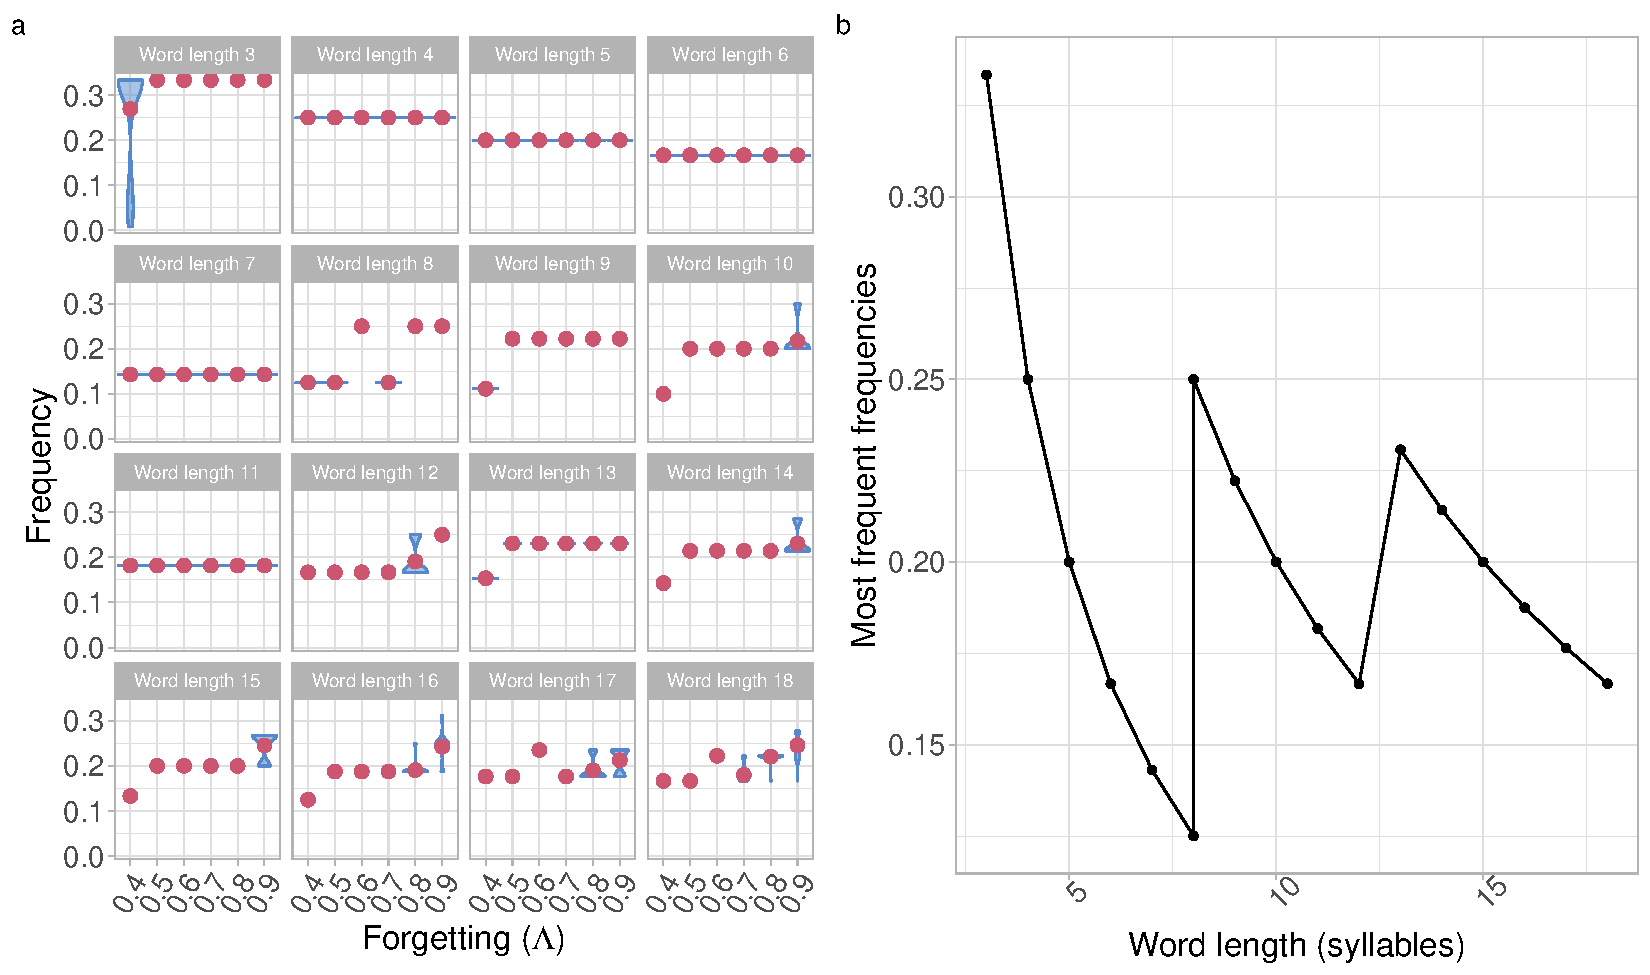
\includegraphics[width=1\linewidth]{tp_model_entrainment_files/figure-latex/basic-experiment-global-by-n-syll-create-freq-plot-plot-1} \caption{Entrainment as a function of word-length. (a) Dominant frequency as a function of the forgetting rate (x-axix, $\Lambda$) and the word-length (3-18 syllables; facets). (b) Most frequent dominant frequency across forgetting rates as a function of the word-length. For words of up to and including 8 syllables, the network entrains to a frequency equivalent to the word-length. For words of 8 or more syllable, the network entrains to a multiple of that frequency.}\label{fig:basic-experiment-global-by-n-syll-create-freq-plot-plot}
\end{figure}

\clearpage

\hypertarget{discussion}{%
\section{Discussion}\label{discussion}}

To acquire the words of their native language, learners need to extract
them from fluent speech, and might use co-occurrence statistics such as
TPs to do so. If so, high-TP items should be stored in memory for later
use as words. Strong evidence in favor of this possibility comes from
electrophysiology, where rhythmic activity has been observed in response
to statistically structured sequences. In the time domain, different
authors have observed amplitude peaks around the boundaries of
statistically defined words
\citep{Abla2008, Cunillera2006, Kudo2011, Sanders2002, Teinonen2009}; in
the frequency domain, a frequency response with a period of the word
duration emerges as participants learn the statistical structure of the
speech stream
\citep{Buiatti2009, Batterink2017, Flo2022, Kabdebon2015, Moreau2022, Moser2021}.

Here, I show that such results can be explained by a simple Hebbian
learning model. When exposed to statistically structured sequences, the
network activation increased towards the end of words due to increased
excitatory input from second order associations. As a result, the
network exhibits rhythmic activity with a period of a word duration.
Critically, given that the network could reproduce these results in the
absence of memory representations for words, earlier
electrophysiological results might also index the statistical
predictability of syllables rather than the acquisition of coherent
units such as words. For example, and as mentioned above, N400 effects
observed in statistical learning tasks
\citep{Abla2008, Cunillera2006, Kudo2011, Sanders2002, Teinonen2009}
might not index the onset of words, but rather the lack of
predictability of word-initial syllables (or the increased
predictability of word-final syllables). This would also be more
consistent with the initial description of the N400 component as an ERP
component that indexes \emph{unpredictable} events \citep{Kutas2000}.

As mention in the introduction, the view that statistical learning does
not necessarily lead to storage in declarative memory memory is
consistent with long-established dissociations between declarative
memory and implicit learning
\citetext{\citealp{Cohen1980}; \citealp{Finn2016}; \citealp[\citet{Knowlton1996a}]{Graf1984}; \citealp{Poldrack2001}; \citealp{Squire1992}}.
It is also consistent with a variety of behavioral results (see
\citep[\citet{Endress-stat-recall}]{Endress2020} for critical reviews),
including behavioral preferences for unattested high-TP items
\citep{Endress-Action-Axc, Endress-Phantoms-Vision, Endress-Phantoms, Jones2007, Turk-Browne-reversal}),
and the inability of adult learners to repeat back words from
familiarization streams with as few as four
words\citep{Endress-stat-recall}.

To identify words in fluent speech, learners might thus need to rely on
other cues, including using known words as cues to word boundaries for
other words \citep{Bortfeld2005, Brent2001, Mersad2012}, paying
attention to beginnings and ends of utterances
\citep{Monaghan2010, Seidl2008, Shukla2007}, phonotactic regularities
\citep{McQueen1998} and universal aspects of prosody
\citep{Brentari2011, Christophe2001, Endress-cross-seg, Pilon1981}.
Computational results suggest that such cues are promising, given that a
computational model attending to utterance edges showed excellent
segmentation and word-learning abilities \citep{Monaghan2010}.

In contrast, statistical learning might well be important for predicting
events across time
\citep{Endress-stat-recall, Morgan2019, Sherman2020, Turk-Browne2010, Verosky2021}
and space \citep{Theeuwes2022}, an ability that is clearly critical for
mature language processing \citep{Levy2008, Trueswell1999} (as well as
many other processes \citep{Clark2013, Friston2010, Keller2018}). This
suggests the possibility that predictive processing might also be
crucial for word learning, but it is an important topic for further
research to find out how predictive processing interacts with language
acquisition.

\clearpage

\hypertarget{supplementary-information}{%
\section{Supplementary Information}\label{supplementary-information}}

\hypertarget{supplementary-information-1-model-definition}{%
\subsection{Supplementary Information 1: Model
definition}\label{supplementary-information-1-model-definition}}

The activation of the \(i^{th}\) unit is given by

\[
\dot{x_i} = -\lambda_a x_i + \alpha \sum_{j \neq i} w_{ij} F(x_j) - \beta \sum_{j \neq i} F(x_j) + \text{noise}
\]

where \(F(x)\) is some activation function. The current simulations use
the function \(F(x) = \frac{x}{1 + x}\). The first term represents
exponential forgetting with a time constant of \(\lambda_a\), the second
term activation from other units, and the third term inhibition among
items to keep the overall activation in a reasonable range.

The weights \(w_{ij}\) are updated using a Hebbian learning rule

\[
\dot{w}_{ij} = - \lambda_w w_{ij} + \rho F(x_i) F(x_j) 
\]

\(\lambda_w\) is the time constant of forgetting (which I set to zero in
the current simulations) while \(\rho\) is the learning rate.

A discrete version of the activation equation is given by

\[
x_i (t+1) = x_i (t) - \lambda_a x_i(t) + \alpha \sum_{j \neq i} w_{ij} F(x_j) - \beta \sum_{j \neq i} F(x_j) + \text{noise}
\]

While the time step is arbitrary in the absence of external input (see
\citep{Endress-Catastrophic-Interference} for a proof), I use the
duration of individual units (e.g., syllables, visual symbols etc.) as
the time unit in the discretization as associative learning is generally
invariant under temporal scaling of the experiment
\citep{Gallistel2000PsychRev, Gallistel2001b}. Further, while only
excitatory connections are tuned by learning in our model, the same
effect could be obtained by tuning inhibition, for example through
tunable disinhibitory interneurons \citep{Letzkus2011}. Here, I simply
focus on the result that a fairly generic network architecture accounts
for rhythmic network activity in response to statistically structured
sequences.

The discrete updating rule for the weights is

\[
w_{ij} (t+1) = w_{ij} (t) - \lambda_w w_{ij} (t) + \rho F(x_i) F(x_j) 
\]

Simulation parameters are listed in Table \ref{tab:params}. An \emph{R}
implementation is available at XXX.

\begin{table}

\caption{\label{tab:list-parameters2}\label{tab:params}Parameters used in the simulations XXX BEAUTIFY AS IN ORIGINAL PAPER}
\centering
\begin{tabular}[t]{ll}
\toprule
Name & Value\\
\midrule
A & 0.7\\
B & 0.4\\
L\_ACT & 0.1, 0.2, 0.3, 0.4, 0.5, 0.6, 0.7, 0.8, 0.9\\
L\_ACT\_DEFAULT & 0.5\\
L\_ACT\_SAMPLES & 0.1, 0.2, 0.3, 0.4, 0.5, 0.6, 0.7, 0.8, 0.9\\
\addlinespace
L\_W & 0\\
N\_ITEMS\_BEFORE\_ACTIVATION\_INSPECTION & 600\\
N\_NEURONS & 19\\
N\_REP\_PER\_WORD & 100\\
N\_REP\_PER\_WORD\_BURNIN & 50\\
\addlinespace
N\_SIM & 100\\
N\_SYLL\_PER\_WORD & 3\\
N\_WORDS & 4\\
NOISE\_SD\_ACT & 0.001\\
NOISE\_SD\_W & 0\\
\addlinespace
R & 0.05\\
\bottomrule
\end{tabular}
\end{table}

\clearpage

\hypertarget{supplementary-information-2-detailed-results}{%
\subsection{Supplementary Information 2: Detailed
results}\label{supplementary-information-2-detailed-results}}

\hypertarget{activation-differences-between-words-and-part-words}{%
\subsubsection{Activation differences between words and
part-words}\label{activation-differences-between-words-and-part-words}}

Table \ref{tab:basic-experiment-global-evaluate-diff-print2} provides
detailed results for the simulations in terms of descriptive statistics
and statistical tests for the simulation testing the recognition of
words and part-words.

\begin{longtable}[t]{llll}
\caption{\label{tab:basic-experiment-global-evaluate-diff-print2}Detailed results for the different forgetting rates and the word vs. part-word comparison (*ABC* vs. *BC:D* and *ABC* vs. *C:DE*), using the global activation as a measure of the network's familiarity with the items. $p_{Wilcoxon}$ represents the *p* value of a Wilcoxon test on the difference scores against the chance level of zero. $P_{Simulations}$ represents the proportion of simulations showing positive difference scores.}\\
\toprule
$\lambda_a$ & Statistic & ABC vs BC:D & ABC vs C:DE\\
\midrule
\endfirsthead
\caption[]{Detailed results for the different forgetting rates and the word vs. part-word comparison (*ABC* vs. *BC:D* and *ABC* vs. *C:DE*), using the global activation as a measure of the network's familiarity with the items. $p_{Wilcoxon}$ represents the *p* value of a Wilcoxon test on the difference scores against the chance level of zero. $P_{Simulations}$ represents the proportion of simulations showing positive difference scores. \textit{(continued)}}\\
\toprule
$\lambda_a$ & Statistic & ABC vs BC:D & ABC vs C:DE\\
\midrule
\endhead

\endfoot
\bottomrule
\endlastfoot
\cellcolor{gray!6}{${100}\times 10^{-3}$} & \cellcolor{gray!6}{{\em M}} & \cellcolor{gray!6}{${-17.1}\times 10^{-3}$} & \cellcolor{gray!6}{${-41.0}\times 10^{-3}$}\\
${100}\times 10^{-3}$ & {\em SE} & ${-1.72}\times 10^{-3}$ & ${-4.12}\times 10^{-3}$\\
\cellcolor{gray!6}{${100}\times 10^{-3}$} & \cellcolor{gray!6}{$p_{Wilcoxon}$} & \cellcolor{gray!6}{${178}\times 10^{-3}$} & \cellcolor{gray!6}{${6.50}\times 10^{-3}$}\\
${100}\times 10^{-3}$ & $P_{Simulations}$ & ${440}\times 10^{-3}$ & ${380}\times 10^{-3}$\\
\cellcolor{gray!6}{${200}\times 10^{-3}$} & \cellcolor{gray!6}{{\em M}} & \cellcolor{gray!6}{${6.44}\times 10^{-3}$} & \cellcolor{gray!6}{${-66.4}\times 10^{-3}$}\\
\addlinespace
${200}\times 10^{-3}$ & {\em SE} & ${647}\times 10^{-6}$ & ${-6.68}\times 10^{-3}$\\
\cellcolor{gray!6}{${200}\times 10^{-3}$} & \cellcolor{gray!6}{$p_{Wilcoxon}$} & \cellcolor{gray!6}{${622}\times 10^{-3}$} & \cellcolor{gray!6}{${2.49}\times 10^{-3}$}\\
${200}\times 10^{-3}$ & $P_{Simulations}$ & ${500}\times 10^{-3}$ & ${320}\times 10^{-3}$\\
\cellcolor{gray!6}{${300}\times 10^{-3}$} & \cellcolor{gray!6}{{\em M}} & \cellcolor{gray!6}{${5.78}\times 10^{-3}$} & \cellcolor{gray!6}{${-16.6}\times 10^{-3}$}\\
${300}\times 10^{-3}$ & {\em SE} & ${581}\times 10^{-6}$ & ${-1.67}\times 10^{-3}$\\
\addlinespace
\cellcolor{gray!6}{${300}\times 10^{-3}$} & \cellcolor{gray!6}{$p_{Wilcoxon}$} & \cellcolor{gray!6}{${123}\times 10^{-3}$} & \cellcolor{gray!6}{${900}\times 10^{-3}$}\\
${300}\times 10^{-3}$ & $P_{Simulations}$ & ${350}\times 10^{-3}$ & ${640}\times 10^{-3}$\\
\cellcolor{gray!6}{${400}\times 10^{-3}$} & \cellcolor{gray!6}{{\em M}} & \cellcolor{gray!6}{${-4.18}\times 10^{-3}$} & \cellcolor{gray!6}{${71.0}\times 10^{-3}$}\\
${400}\times 10^{-3}$ & {\em SE} & ${-420}\times 10^{-6}$ & ${7.14}\times 10^{-3}$\\
\cellcolor{gray!6}{${400}\times 10^{-3}$} & \cellcolor{gray!6}{$p_{Wilcoxon}$} & \cellcolor{gray!6}{${193}\times 10^{-18}$} & \cellcolor{gray!6}{${3.96}\times 10^{-18}$}\\
\addlinespace
${400}\times 10^{-3}$ & $P_{Simulations}$ & ${90.0}\times 10^{-3}$ & $1.00$\\
\cellcolor{gray!6}{${500}\times 10^{-3}$} & \cellcolor{gray!6}{{\em M}} & \cellcolor{gray!6}{${3.98}\times 10^{-3}$} & \cellcolor{gray!6}{${63.7}\times 10^{-3}$}\\
${500}\times 10^{-3}$ & {\em SE} & ${400}\times 10^{-6}$ & ${6.40}\times 10^{-3}$\\
\cellcolor{gray!6}{${500}\times 10^{-3}$} & \cellcolor{gray!6}{$p_{Wilcoxon}$} & \cellcolor{gray!6}{${38.1}\times 10^{-18}$} & \cellcolor{gray!6}{${3.96}\times 10^{-18}$}\\
${500}\times 10^{-3}$ & $P_{Simulations}$ & ${930}\times 10^{-3}$ & $1.00$\\
\addlinespace
\cellcolor{gray!6}{${600}\times 10^{-3}$} & \cellcolor{gray!6}{{\em M}} & \cellcolor{gray!6}{${7.54}\times 10^{-3}$} & \cellcolor{gray!6}{${50.6}\times 10^{-3}$}\\
${600}\times 10^{-3}$ & {\em SE} & ${758}\times 10^{-6}$ & ${5.08}\times 10^{-3}$\\
\cellcolor{gray!6}{${600}\times 10^{-3}$} & \cellcolor{gray!6}{$p_{Wilcoxon}$} & \cellcolor{gray!6}{${3.96}\times 10^{-18}$} & \cellcolor{gray!6}{${3.96}\times 10^{-18}$}\\
${600}\times 10^{-3}$ & $P_{Simulations}$ & $1.00$ & $1.00$\\
\cellcolor{gray!6}{${700}\times 10^{-3}$} & \cellcolor{gray!6}{{\em M}} & \cellcolor{gray!6}{${9.58}\times 10^{-3}$} & \cellcolor{gray!6}{${28.1}\times 10^{-3}$}\\
\addlinespace
${700}\times 10^{-3}$ & {\em SE} & ${963}\times 10^{-6}$ & ${2.83}\times 10^{-3}$\\
\cellcolor{gray!6}{${700}\times 10^{-3}$} & \cellcolor{gray!6}{$p_{Wilcoxon}$} & \cellcolor{gray!6}{${3.96}\times 10^{-18}$} & \cellcolor{gray!6}{${3.96}\times 10^{-18}$}\\
${700}\times 10^{-3}$ & $P_{Simulations}$ & $1.00$ & $1.00$\\
\cellcolor{gray!6}{${800}\times 10^{-3}$} & \cellcolor{gray!6}{{\em M}} & \cellcolor{gray!6}{${9.46}\times 10^{-3}$} & \cellcolor{gray!6}{${17.2}\times 10^{-3}$}\\
${800}\times 10^{-3}$ & {\em SE} & ${950}\times 10^{-6}$ & ${1.73}\times 10^{-3}$\\
\addlinespace
\cellcolor{gray!6}{${800}\times 10^{-3}$} & \cellcolor{gray!6}{$p_{Wilcoxon}$} & \cellcolor{gray!6}{${3.96}\times 10^{-18}$} & \cellcolor{gray!6}{${3.96}\times 10^{-18}$}\\
${800}\times 10^{-3}$ & $P_{Simulations}$ & $1.00$ & $1.00$\\
\cellcolor{gray!6}{${900}\times 10^{-3}$} & \cellcolor{gray!6}{{\em M}} & \cellcolor{gray!6}{${5.42}\times 10^{-3}$} & \cellcolor{gray!6}{${7.63}\times 10^{-3}$}\\
${900}\times 10^{-3}$ & {\em SE} & ${545}\times 10^{-6}$ & ${767}\times 10^{-6}$\\
\cellcolor{gray!6}{${900}\times 10^{-3}$} & \cellcolor{gray!6}{$p_{Wilcoxon}$} & \cellcolor{gray!6}{${3.96}\times 10^{-18}$} & \cellcolor{gray!6}{${3.96}\times 10^{-18}$}\\
\addlinespace
${900}\times 10^{-3}$ & $P_{Simulations}$ & $1.00$ & $1.00$\\*
\end{longtable}

\clearpage

\hypertarget{electrophysiological-results-1}{%
\subsubsection{Electrophysiological
results}\label{electrophysiological-results-1}}

\hypertarget{activation-differences-within-words.}{%
\paragraph{Activation differences within
words.}\label{activation-differences-within-words.}}

Table \ref{tab:basic-experiment-global-print-act-in-words-table2} shows
activation differences between pairs of neurons in different positions
within words.

\begin{table}

\caption{\label{tab:basic-experiment-global-print-act-in-words-table2}Difference scores between syllable activations in different positions. P values reflect a Wilcoxon test against the chance level of zero.}
\centering
\begin{tabular}[t]{rrrrrrrrrr}
\toprule
\multicolumn{1}{c}{ } & \multicolumn{3}{c}{$\sigma_2 - \sigma_1$} & \multicolumn{3}{c}{$\sigma_3 - \sigma_2$} & \multicolumn{3}{c}{$\sigma_3 - \sigma_1$} \\
\cmidrule(l{3pt}r{3pt}){2-4} \cmidrule(l{3pt}r{3pt}){5-7} \cmidrule(l{3pt}r{3pt}){8-10}
$\Lambda$ & M & SE & p & M & SE & p & M & SE & p\\
\midrule
0.4 & -0.1773874 & 0.0006361 & 0 & 0.0704068 & 0.0009216 & 0 & -0.1069806 & 0.0013369 & 0\\
0.5 & -0.1844972 & 0.0003990 & 0 & 0.1690059 & 0.0002893 & 0 & -0.0154913 & 0.0001735 & 0\\
0.6 & -0.0887014 & 0.0002317 & 0 & 0.1435672 & 0.0002364 & 0 & 0.0548658 & 0.0000747 & 0\\
0.7 & 0.0120559 & 0.0000503 & 0 & 0.0668735 & 0.0001011 & 0 & 0.0789294 & 0.0000659 & 0\\
0.8 & 0.0237136 & 0.0000256 & 0 & 0.0322450 & 0.0000630 & 0 & 0.0559587 & 0.0000539 & 0\\
\addlinespace
0.9 & 0.0198019 & 0.0000211 & 0 & 0.0075441 & 0.0000225 & 0 & 0.0273459 & 0.0000265 & 0\\
\bottomrule
\end{tabular}
\end{table}

\clearpage

\hypertarget{number-of-active-neurons}{%
\paragraph{Number of active neurons}\label{number-of-active-neurons}}

Table \ref{tab:inspect-number-of-active-neurons-print2} and Figure
\ref{fig:inspect-number-of-active-neurons-plot2} show the number of
simultaneously active neurons as a function of the forgetting rate.

\begin{table}

\caption{\label{tab:inspect-number-of-active-neurons-print2}Number of simultaneously  active neurons as a function of the forgetting rate.}
\centering
\begin{tabular}[t]{rrr}
\toprule
$\Lambda$ & M & SE\\
\midrule
0.1 & 3.869 & 0.061\\
0.2 & 3.962 & 0.028\\
0.3 & 3.611 & 0.006\\
0.4 & 3.199 & 0.002\\
0.5 & 2.997 & 0.001\\
\addlinespace
0.6 & 2.500 & 0.001\\
0.7 & 2.031 & 0.000\\
0.8 & 2.000 & 0.000\\
0.9 & 2.000 & 0.000\\
\bottomrule
\end{tabular}
\end{table}

\begin{figure}
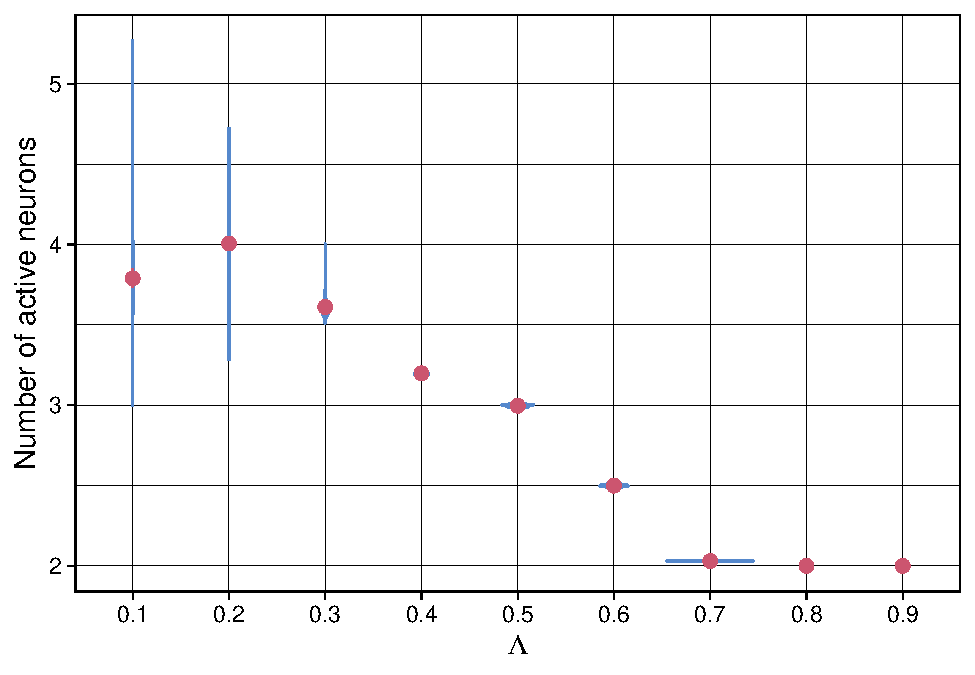
\includegraphics[width=1\linewidth]{tp_model_entrainment_files/figure-latex/inspect-number-of-active-neurons-plot2-1} \caption{Average number of simultaneously active neurons as a function of the forgetting rate.}\label{fig:inspect-number-of-active-neurons-plot2}
\end{figure}

\clearpage

\hypertarget{spectral-density-1}{%
\subsubsection{Spectral density}\label{spectral-density-1}}

\hypertarget{phase-analysis-1}{%
\subsubsection{Phase analysis}\label{phase-analysis-1}}

Table \ref{tab:basic-experiment-global-phase-table2} shows the
descriptives of the relative phase of the network activation relative to
the different syllable positions.

\begin{table}

\caption{\label{tab:basic-experiment-global-phase-table2}Relative phases of the network activation relative to different syllable positions in degrees.}
\centering
\begin{tabular}[t]{rrrrrrrrr}
\toprule
\multicolumn{1}{c}{ } & \multicolumn{8}{c}{Phase in degrees relative to} \\
\cmidrule(l{3pt}r{3pt}){2-9}
\multicolumn{1}{c}{ } & \multicolumn{2}{c}{$\sigma_1$} & \multicolumn{2}{c}{$\sigma_2$} & \multicolumn{2}{c}{$\sigma_3$} & \multicolumn{2}{c}{Saw tooth} \\
\cmidrule(l{3pt}r{3pt}){2-3} \cmidrule(l{3pt}r{3pt}){4-5} \cmidrule(l{3pt}r{3pt}){6-7} \cmidrule(l{3pt}r{3pt}){8-9}
$\Lambda$ & M & SE & M & SE & M & SE & M & SE\\
\midrule
0.4 & 19.84307 & 3.7407781 & 121.99719 & 6.5897001 & -87.727138 & 4.3081432 & -111.342035 & 5.7277658\\
0.5 & 55.75048 & 0.0438438 & 175.75048 & 0.0438438 & -64.249518 & 0.0438438 & -94.249517 & 0.0438438\\
0.6 & 82.02099 & 0.0471422 & -157.97901 & 0.0471422 & -37.979008 & 0.0471422 & -67.979007 & 0.0471422\\
0.7 & 128.42569 & 0.0423470 & -111.57431 & 0.0423470 & 8.425687 & 0.0423470 & -21.574313 & 0.0423470\\
0.8 & 145.05601 & 0.0442561 & -94.94399 & 0.0442561 & 25.056007 & 0.0442561 & -4.943993 & 0.0442561\\
\addlinespace
0.9 & 164.62347 & 0.0415040 & -75.37653 & 0.0415040 & 44.623472 & 0.0415040 & 14.623472 & 0.0415040\\
\bottomrule
\end{tabular}
\end{table}

\clearpage

\hypertarget{memory-for-word-onsets-vs.-offsets}{%
\subsubsection{Memory for word-onsets
vs.~offsets}\label{memory-for-word-onsets-vs.-offsets}}

Table
\ref{tab:basic-experiment-global-print-difference-between-parts-of-word2}
shows the descriptives of activation differences between syllable
bigrams at word onsets and word offsets, respectively.

\begin{table}

\caption{\label{tab:basic-experiment-global-print-difference-between-parts-of-word2}Activation difference between items composed of the first two syllables of a word and the last two syllables of a word, when these bigrams were presented in isolation. Positive values indicate greater activation for the AB items than the BC items. The p value reflects a two-sided Wilcoxon signed rank test against the chance level of zero}
\centering
\begin{tabular}[t]{rrrr}
\toprule
\multicolumn{1}{c}{ } & \multicolumn{3}{c}{Activation difference between AB and BC items} \\
\cmidrule(l{3pt}r{3pt}){2-4}
$\Lambda$ & M & SE & p\\
\midrule
0.1 & -0.9994440 & 0.7955509 & 0.2063792\\
0.2 & 0.5624835 & 0.4675769 & 0.6786411\\
0.3 & -0.1798655 & 0.0454490 & 0.0000000\\
0.4 & -0.1542890 & 0.0034314 & 0.0000000\\
0.5 & -0.0657494 & 0.0004952 & 0.0000000\\
\addlinespace
0.6 & -0.0370576 & 0.0003829 & 0.0000000\\
0.7 & -0.0189230 & 0.0003555 & 0.0000000\\
0.8 & -0.0107695 & 0.0003299 & 0.0000000\\
0.9 & -0.0034387 & 0.0003085 & 0.0000000\\
\bottomrule
\end{tabular}
\end{table}

\hypertarget{positional-similarity-new-in-revision}{%
\subsubsection{Positional similarity (NEW IN
REVISION)}\label{positional-similarity-new-in-revision}}

Table \ref{tab:basic-similarity-by-position-print-difference2} shows the
descriptives of the relative difference in cosine similarity for pairs
of representations mismatching and matching in the their sequential
positions, respectively

\begin{table}

\caption{\label{tab:basic-similarity-by-position-print-difference2}Simulations of positional codes cite{Henin2021}. Representations of syllables *not* sharing a sequential position (i.e., word-initial, word-medial, word-final) are more similar to each other than representations of syllables sharing a sequential position. The similarity was evaluated using the cosine similarity across the vectors of activation elicited by the syllables. The p value reflects a Wilcoxon test against the chance level of zero.}
\centering
\begin{tabular}[t]{rrrr}
\toprule
\multicolumn{1}{c}{ } & \multicolumn{3}{c}{Relative cosine similarity difference \$\textbackslash{}frac\{Non-match - Match\}\{Non-match + Match\}\$} \\
\cmidrule(l{3pt}r{3pt}){2-4}
$\Lambda$ & M & SE & p\\
\midrule
0.1 & 0.0000480 & 0.0000052 & 0\\
0.2 & 0.0000670 & 0.0000087 & 0\\
0.3 & 0.0047546 & 0.0023126 & 0\\
0.4 & 0.4537155 & 0.0019926 & 0\\
0.5 & 0.6514078 & 0.0004043 & 0\\
\addlinespace
0.6 & 0.7223419 & 0.0002397 & 0\\
0.7 & 0.8021107 & 0.0001836 & 0\\
0.8 & 0.8815936 & 0.0001086 & 0\\
0.9 & 0.9475520 & 0.0000458 & 0\\
\bottomrule
\end{tabular}
\end{table}

\hypertarget{heard-vs.-unheard-items-flo2022-new-in-revision}{%
\subsubsection{\texorpdfstring{Heard vs.~unheard items \citep{Flo2022}
(NEW IN
REVISION)}{Heard vs.~unheard items {[}@Flo2022{]} (NEW IN REVISION)}}\label{heard-vs.-unheard-items-flo2022-new-in-revision}}

While the current model provides a qualitative explanation of a number
of statistical learning results, it is unlikely to make quantitative
predictions. A case in point are some test items used by
\citep{Flo2022}. Specifically, they sought ERP responses to TP
violations by pitting hear items against non-heard items.

The heard items were words (of the form \(A_iB_iC_i\)) and part-words
(of the form \(B_iC_iA_k\)). The unheard items were edge-words (of the
form \(A_iB_iC_k\)) and non-words (of the form \(B_iC_iA_i\)). While
\citep{Flo2022} did not observe significant ERP differences between
these item types, modeling this null effect likely requires quantitative
predictions of different cues that might drive such differences (apart
from issues associated with modeling null effects).

Specifically, while the forward and backward TPs are stronger in heard
items than in un-heard items, this description of the test items depends
on calculating TPs at a constant lag. For example, in edge-words
(\(A_iB_iC_k\)), the \(C_k\) syllable is associated with the other
syllables, given that participants encountered part-words such as
\(C_kA_iB_i\). Likewise, in non-words (\(B_iC_iA_i\)), all syllables are
strongly associated with one another, given that the item is a scrambled
version of a word \(A_iB_iC_i\). Depending on how learners integrate
associations across directions (forward or backward) and lags, they
might or might not differentiate \citep{Flo2022} heard items from their
unheard items.

In contrast to \citep{Flo2022} results, Figure
\ref{fig:basic-experiment-global-print-act-3syll-flo2022-plot} and Table
\ref{tab:basic-experiment-global-print-difference-between-3syll-items-from-flo2022}
show that, with the current parameter set, the network prefers heard
items over unheard items for forgetting rates of at least 0.4. However,
these results likely depend on the interplay between forgetting,
excitation, interference as well as the structure of the speech stream.

\begin{figure}
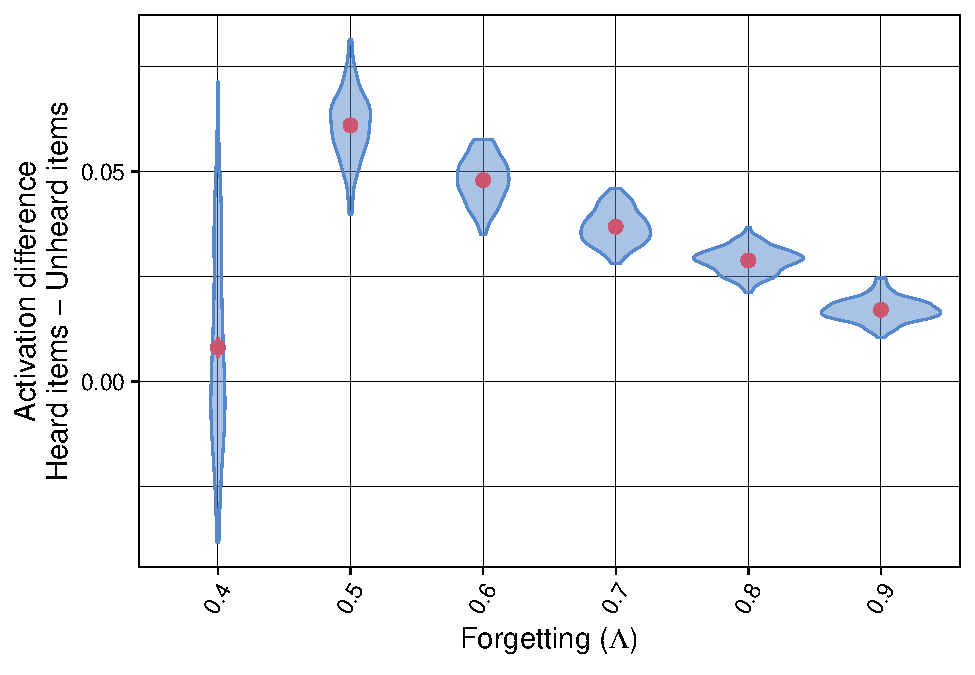
\includegraphics[width=1\linewidth]{tp_model_entrainment_files/figure-latex/basic-experiment-global-print-act-3syll-flo2022-plot-1} \caption{Average difference in the total network activation for the heard item ($A_iB_iC_i$ and $B_iC_iA_k$) vs. unheard item contrast ($A_iB_iC_k$; $B_iC_iA_i$) used by cite{Flo2022}. The results reflect the network behavior after the first 50 presentations of each word. Positive values indicate greater activation for the heard items than the unheard items.}\label{fig:basic-experiment-global-print-act-3syll-flo2022-plot}
\end{figure}

\begin{table}

\caption{\label{tab:basic-experiment-global-print-difference-between-3syll-items-from-flo2022}Average difference in the total network activation for the heard item ($A_iB_iC_i$ and $B_iC_iA_k$) vs. unheard item contrast ($A_iB_iC_k$; $B_iC_iA_i$) used by cite{Flo2022}. The results reflect the network behavior after the first 50 presentations of each word. Positive values indicate greater activation for the heard items than the unheard items. The p value reflects a two-sided Wilcoxon signed rank test against the chance level of zero}
\centering
\begin{tabular}[t]{rrrr}
\toprule
\multicolumn{1}{c}{ } & \multicolumn{3}{c}{Activation difference between heard items and unheard items} \\
\cmidrule(l{3pt}r{3pt}){2-4}
\$\textbackslash{}Lambda\$ & M & SE & p\\
\midrule
0.1 & -1.010 & 2.806 & 0.798\\
0.2 & 1.237 & 1.869 & 0.331\\
0.3 & 0.339 & 0.423 & 0.280\\
0.4 & 0.008 & 0.002 & 0.007\\
0.5 & 0.061 & 0.001 & 0.000\\
\addlinespace
0.6 & 0.048 & 0.001 & 0.000\\
0.7 & 0.037 & 0.000 & 0.000\\
0.8 & 0.029 & 0.000 & 0.000\\
0.9 & 0.017 & 0.000 & 0.000\\
\bottomrule
\end{tabular}
\end{table}

  \bibliography{../misc/ansgar.bib}

\end{document}
